\documentclass{article}
\usepackage[utf8]{inputenc}
\usepackage[options ]{algorithm2e}
\usepackage{algorithmic}
\usepackage{algorithm}

\usepackage[english]{babel}
\usepackage[utf8]{inputenc}
\usepackage{amsmath}
\usepackage{amsfonts}
\usepackage{graphicx}
\usepackage[colorinlistoftodos]{todonotes}
\usepackage{algorithm}
\usepackage{algpseudocode}

\title{The Producer Consumer problem}
\author{Diaconescu Bogdan-Florin\\ CR 3.2 A, Anul 3}

\usepackage{natbib}
\usepackage{graphicx}

\begin{document}
\maketitle
\newpage
\section{Problem statement}
\hspace{0.5 cm}
Problema producator-consumator presupune crearea a 2 procese, producatorul si consumatorul care utilizeaza o resursa comuna, cu dimensiune fixa, numita buffer, care se comporta ca si o coada. Rolul producatorului este acelasi de a genera date si de a le introduce in buffer. In acelasi timp, rolul consumatorului este de a "consuma" datele din buffer una cate una. 

\hspace{0.5 cm}
De asemenea, trebuie evitata situatia cand producatorul incearca sa puna date in buffer desi acesta este plin, sau atunci cand consumatorul incearca sa "consume" date din buffer -ul gol. 

\section{Implementation/Solution}
\hspace{0.5 cm}
{\large \textbf {Solutia utilizand monitoare}}

\vspace{5mm}
\hspace{0.5 cm}
Pentru a rezolva problema am creat 2 clase, Produse si Consumer care extind clasa Thread din java, respectiv clasa Market, care reprezinta de fapt buffer -ul. 

\hspace{0.5 cm}
In clasa Market am implementat cele 2 functii produce si consume, iar buffer -ul este reprezentat de un vector de numere intregi de dimensiunea N. Aceste 2 functii sunt de tipul synchronized pentru a ma asigura ca un singur thread poate executa metoda respectiva la un moment dat. In cazul in care buffer -ul este deja plin, in interiorul metodei produce se apeleaza metoda wait(). Aceasta metoda face ca celelalte threaduri care asteapta dupa blocajul aceluiasi obiect sa poata sa intre in lucru. Cu alte cuvinte, prin adaugarea acestei metode se stopeaza producatorul, dar se elibereaza accesul la resursa comuna, adica consumatorul poate sa "consume" date din buffer. Atunci cand este eliberat un loc in buffer, metoda produse este "trezita" prin apelarea metodei notifyAll() de catre consumator.

\hspace{0.5 cm}
In clasele Producer si Consumer metoda run() implementeaza "producerea" si "consumul" datelor. Clasa Main contine functia main in care sunt create threadurile producator si consumator si este pornita executia acestora cu metoda start(). Am utilizat 2 variabile MINN si MAXN pentru a generare producatori si consumatori in intervalul 0-76. La final fiecare consumator si producator afiseaza numarul de elemente "consumate", respectiv "produse".

\vspace{5mm}
{\large \textbf {Solutia utilizand zavoare}}

\hspace{0.5 cm}
Rezolvarea problemei utilizand zavoarele este asemanatoare ca cea cu monitoare. Daca la monitoare blocarea si deblocarea se faceau automat, la zavoare, atat deblocarea cat si blocarea zavorului se face utilizand functiile lock() si unlock(). Singura clasa schimbata este clasa Market, unde metodele produce si consume au fost implementate utilizand functii din biblioteca ReentrantLock din java. Am adaugat si 2 variabile boolene notFull si notEmpty pentru a verifica daca bufferul este plin sau gol, care initial au valorile true, respectiv false. 

\hspace{0.5 cm}
De asemenea, am creat si un zavor numit bufferLock, care la inceputul functiilor procese si consume blocheaza accesul la sectiunea critica prin apelarea functiei lock(). Oricare alt thread care incearca sa apeleze functia lock() va fi blocat pana cand threadul care a apelat functia lock() va debloca bufferLock prin apelul functiei unlock(). La finalul functiilor produce si consume, bufferLock deblocheaza accesul la sectiunea critica prin apelul functiei unlock().

\begin{algorithm} 
\caption{Functia produce implementata cu zavoare}
\algblock[TryCatchFinally]{try}{endtry}
\algcblock[TryCatchFinally]{TryCatchFinally}{finally}{endtry}
\algcblockdefx[TryCatchFinally]{TryCatchFinally}{catch}{endtry}
	[1]{\textbf{catch} #1}
	{\textbf{end try}}
\begin{algorithmic}[1]
\Function{public void produce}{int value}

\STATE bufferLock.lock();
 \try
    \IF {notFull == true}
    \STATE $buffer[newest] \gets value $
    \STATE $newest \gets (newest + 1) \% N $
    \STATE $count++$
    \ENDIF
    \IF {count == N}
    \STATE $notFull \gets false$
    \ENDIF
    \STATE $notEmpty \gets true$
  \finally{}
    \State{bufferLock.unlock()}
  \endtry

\end{algorithmic}
\end{algorithm}

\begin{algorithm} 
\caption{Functia consume implementata cu zavoare}
\algblock[TryCatchFinally]{try}{endtry}
\algcblock[TryCatchFinally]{TryCatchFinally}{finally}{endtry}
\algcblockdefx[TryCatchFinally]{TryCatchFinally}{catch}{endtry}
	[1]{\textbf{catch} #1}
	{\textbf{end try}}
\begin{algorithmic}[1]
\Function{public int consume}{}
\STATE $value \gets -1$
\STATE bufferLock.lock();
 \try
    \IF {notEmpty == true}
    \STATE $value \gets buffer[oldest] $
    \STATE $oldest \gets (oldest + 1) \% N $
    \STATE $count--$
    \ENDIF
    \IF {count == 0}
    \STATE $notEmpty \gets false$
    \ENDIF
    \STATE $notFull \gets true$
  \finally{}
    \State{bufferLock.unlock()}
  \endtry
  \STATE return value

\end{algorithmic}
\end{algorithm}

\newpage
\vspace{5mm}
{\large \textbf {Solutia utilizand semafoare}}

\hspace{0.5 cm}
Am rezolvat problema utilizand biblioteca Semaphore din java pentru implementarea semafoarelor.In clasa Market am creat 4 semafoare: 2 semafoare pentru producator si consumator, producerSemaphore si consumerSemaphore, si 2 semafoare notFull si notEmpty pentru a verifica daca bufferul este plin sau gol. producerSemaphore si notFull primesc initial permisiunea 1, deoarece la inceput producatorul se apeleaza prima data, iar bufferul nu este plin. 

\hspace{0.5 cm}
In functiile produce si consume mai intai se incearca intr-un bloc try catch obtinerea permisiunii de la semafoare. In cazul functiei produse, se cere permisunea de la producerSemaphore si notFull. Daca se primesc permisiunile se trece la adugarea elementului in buffer, in caz contrat se genereaza o exceptie. La final se verifica daca bufferul este plin sau gol si se incrementeaza semafoarele. In mod asemanator este construita si functia consume(). Clasele Producer, Consumer si Main au ramas neschimbate.

\section{Experimental data}
\hspace{0.5 cm}
In rezolvarea problemei utilizand monitoare am folosit, initial, in loc de functia wait(), apelul Thread.currentThread().sleep(6). Insa, in timpul executiei, s-a intamplat fenomenul deadlock, adica 2 threaduri asteptau la infinit unul dupa celalalt, niciunul neputand sa-si continue executia. Aceasta problema a fost rezolvata prin folosirea functiei wait(), care elibereaza blocajul pe un thread, astfel celelalte threaduri care asteapta dupa el putand sa-si continue executia.

\hspace{0.5 cm}
Pentru fiecare mod de rezolvare al problemei am calculat timpul de executie pentru fiecare thread producator si consumator.Timpul mediu cel mai scurt in care toate threadurile si-au incheiat executia a fost obtinut in cazul rezolvarii utilizand monitoarele: 6 milisecunde. Pentru celelalte 2 metode am obtinut urmatorii timpi medii de executie: 10290 milisecunde pentru implementarea utilizand zavoare si 14166 pentru cea cu semafoare.

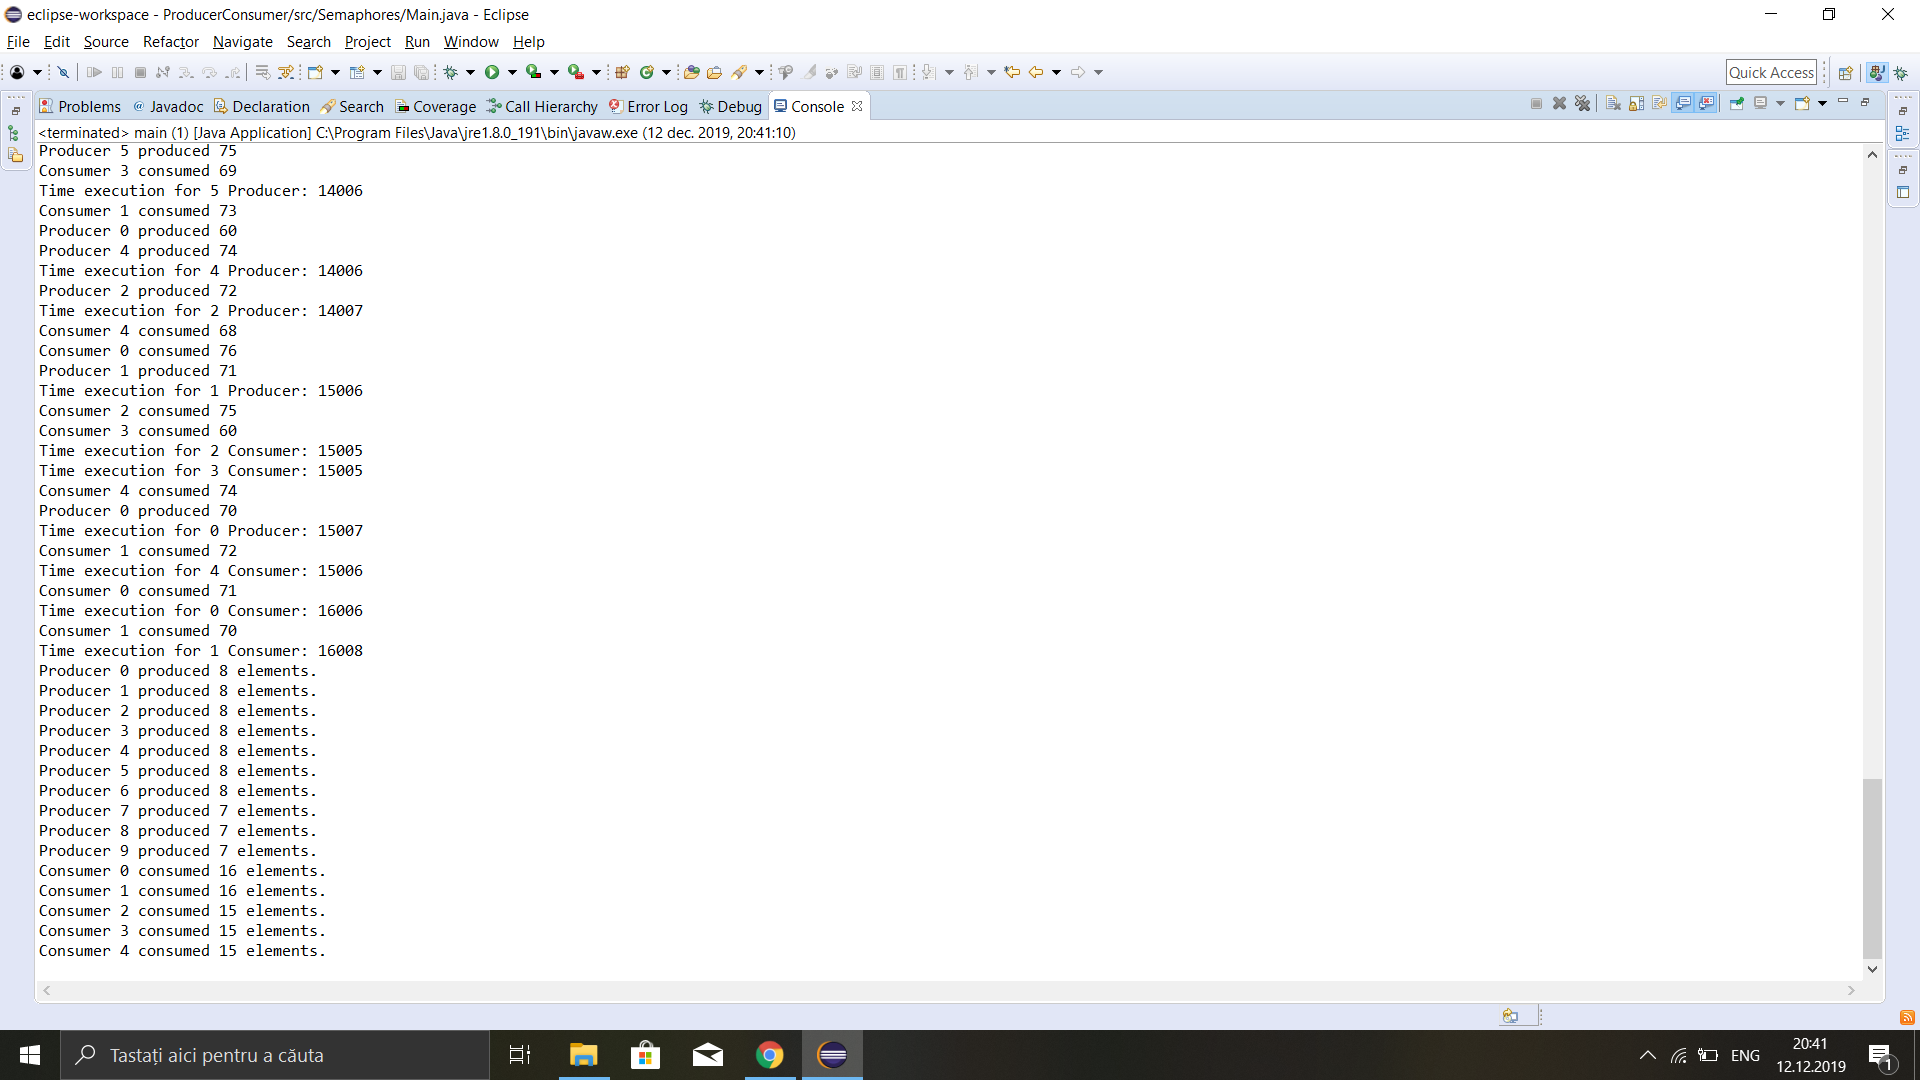
\includegraphics{PCSemaphores.png}
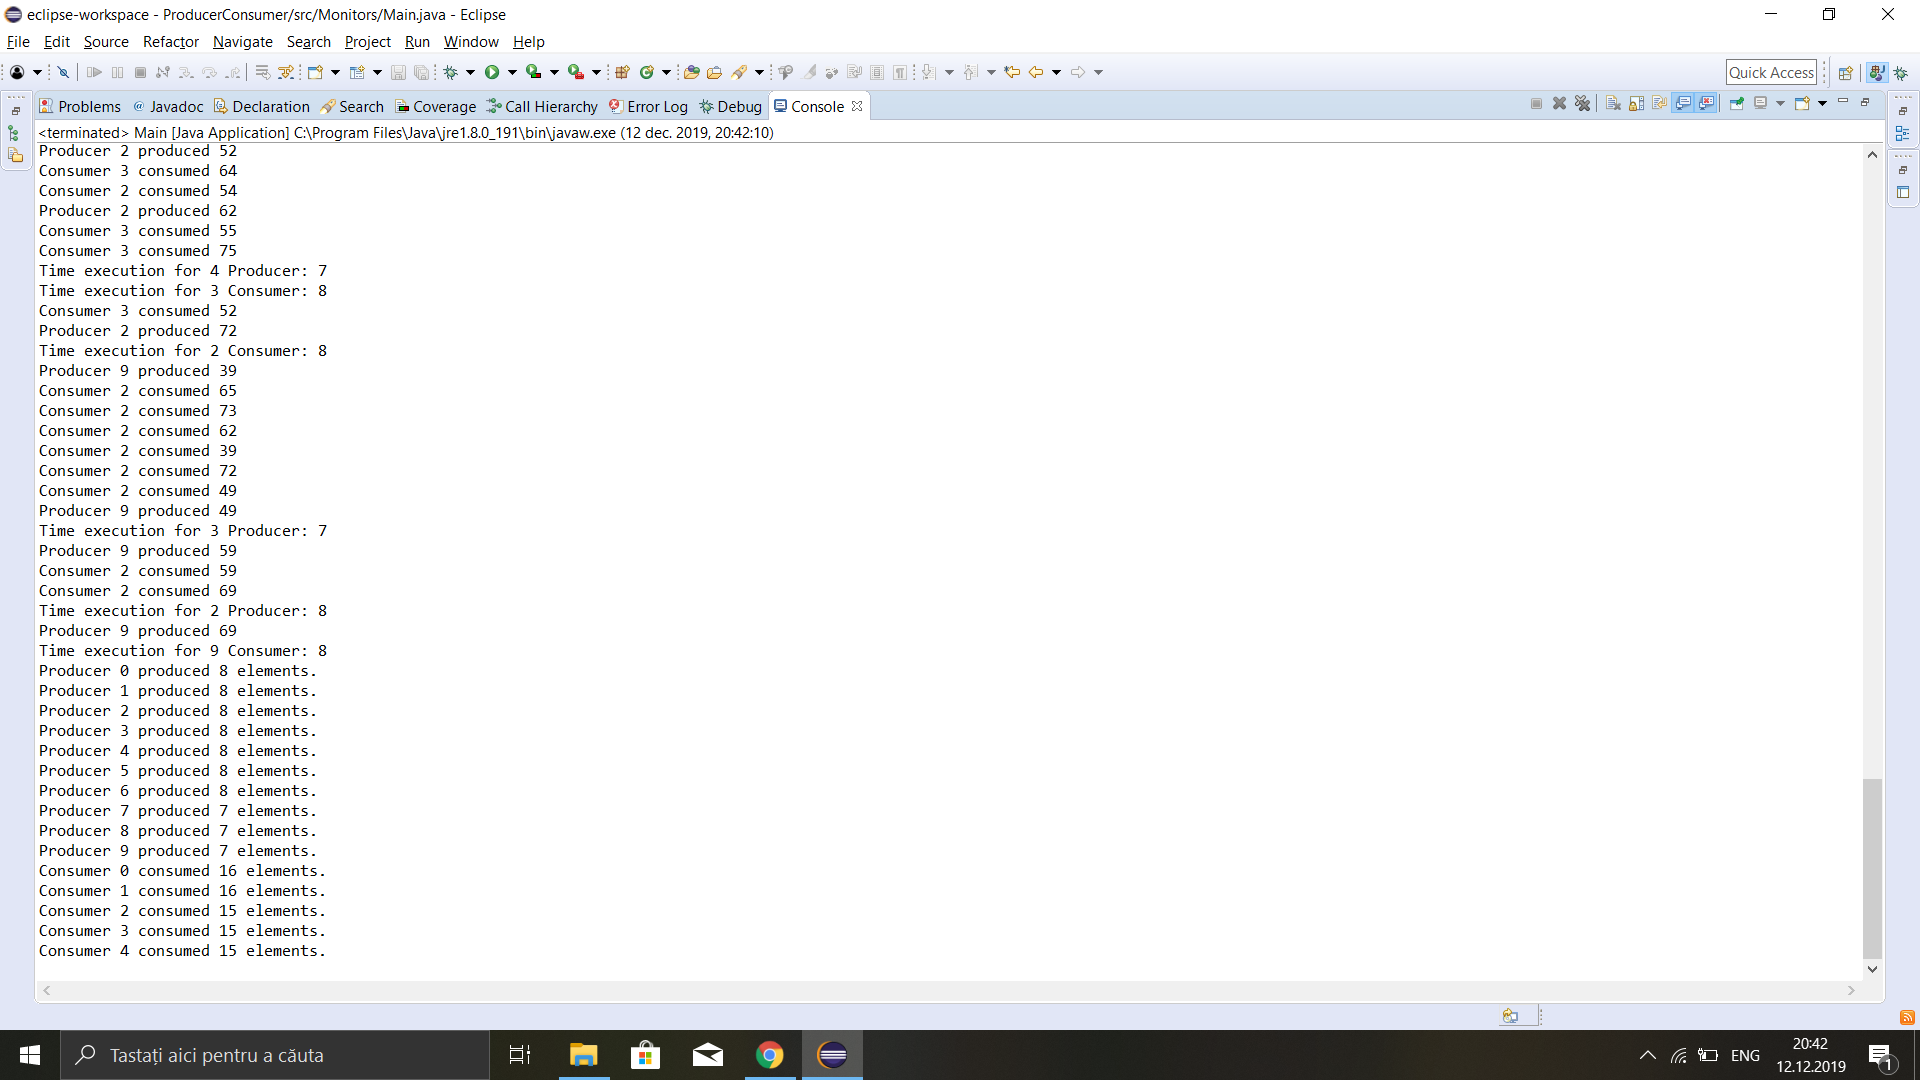
\includegraphics{PCMonitors.png}
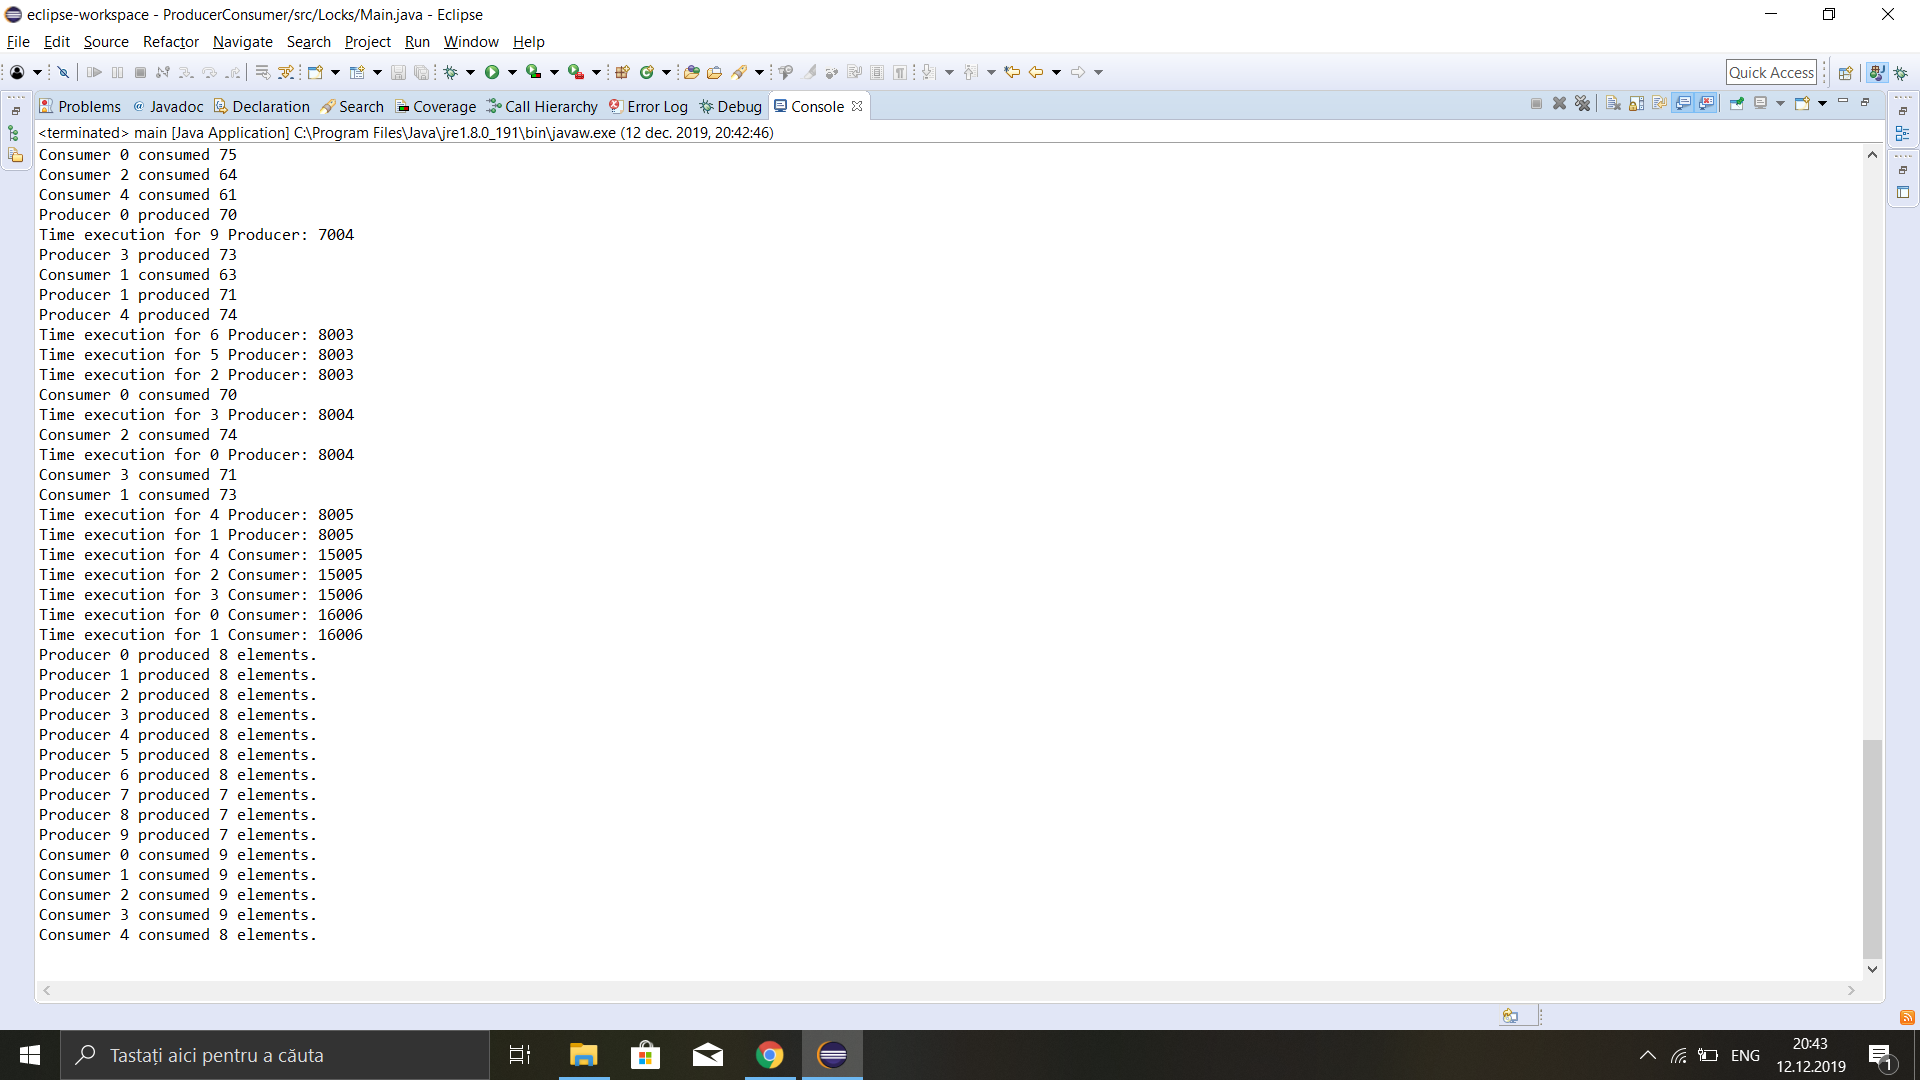
\includegraphics{PCLocks.png}

\section{Results \& Conclusions}
\hspace{0.5 cm}
Cea mai eficienta metoda de rezolvare a problemei Producator-Consumator este cea utilizand monitoarele, prin folosirea mecanismului synchronized pentru functiile produce si consume. Rezolvarea folosind zavoare este asemanatoare cu cea cu monitoare, diferenta consta in faptul ca fiecare thread se blocheaza si se deblocheaza prin apelul functiilor lock() si unlock(), lucru care la monitoare se face automat in timpul executiei. Cea de-a treia metoda de rezolvare, cea in care se utilizeaza semafoare este apropiata ca timp de executie de cea cu zavoare, dar are cel mai mare timp de executie.

\end{document}